\documentclass{beamer}
\usepackage{graphicx}
\graphicspath{ {images/} }

\title[Forum Presentation]{COSC3500 Forum Presentation}
\author{Max Bo}
\date{22nd of October}

\begin{document}

\begin{frame}
  \titlepage
\end{frame}

% The presentations will be marked out of 5 according to the following general criteria:

% General presentation technique (/1.5)

% Depth and detail; comparing commonalities (/2.5)

% Question time: demonstrating correctness of work and understanding of concepts (1)

% Uncomment these lines for an automatically generated outline.
\begin{frame}{Outline}
 \tableofcontents
\end{frame}

% \section{Introduction}

% \begin{frame}{Introduction}

% \begin{itemize}
%   \item Your introduction goes here!
% \end{itemize}

\begin{frame}{Description}
\section{Description}
The task was to create a stock-standard, 2-dimensional gravitational $n$-body simulator. 

\vskip 1cm

All bodies were to be assumed to be point masses. The simulation was to be accurate, maintaining a constant total energy, and exhibiting phenomena such as apsidal precession. 
\end{frame}

\begin{frame}{Demo}
\section{Demo}
\end{frame}

\begin{frame}[allowframebreaks]{Integration}
\section{Integration}

\[
  F = G \frac{m_1 m_2}{r^2}
\]

\begin{align*}
a_{i}&=F(x_{i})\\
v_{i+1}&=v_{i}+a_{i}\,\Delta t\\
\end{align*}

\framebreak

Dehen and Read note that the Euler method `performs very poorly in practice', further noting that `errors are proportional to $\Delta t^2$'. They contrast it with the second-order \textit{Leapfrog} symplectic integrator, which is `heavily used in collisionless N-body applications'.

\begin{align*}
x_{i}&=x_{i-1}+v_{i-1/2}\,\Delta t\\
a_{i}&=F(x_{i})\\
v_{i+1/2}&=v_{i-1/2}+a_{i}\,\Delta t\\
\end{align*}

which only requires a single acceleration calculation per every two half timesteps

\framebreak

and a `kick-drift-kick' form

\begin{align*}
v_{i+1/2}&=v_{i}+a_{i}{\frac {\Delta t}{2}}\\
x_{i+1}&=x_{i}+v_{i+1/2}\Delta t\\
v_{i+1}&=v_{i+1/2}+a_{i+1}{\frac {\Delta t}{2}}
\end{align*}

that is stable with variable timstepping, but incurs an additional acceleration calculation per every two half timesteps.
\end{frame}

\begin{frame}[allowframebreaks]{Barnes-Hut}
\section{Barnes-Hut}

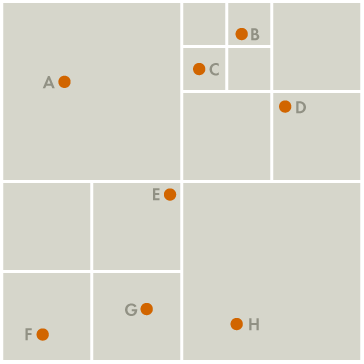
\includegraphics[width=0.6\textwidth]{quadtree}

\framebreak

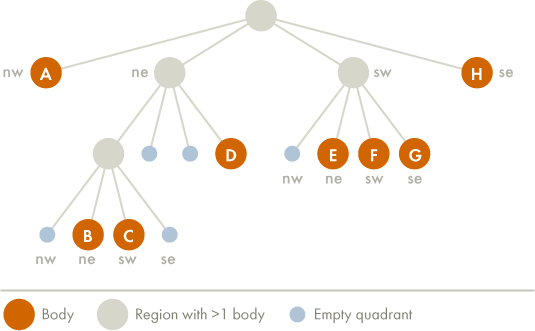
\includegraphics[width=\textwidth]{quadtree_tree}

\framebreak

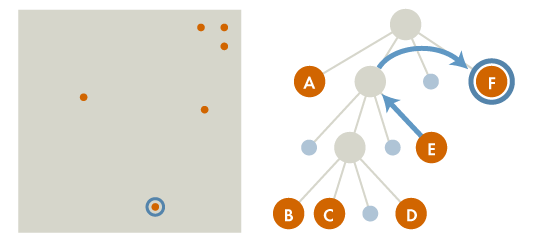
\includegraphics[width=\textwidth]{quadtree_leaf}

\framebreak

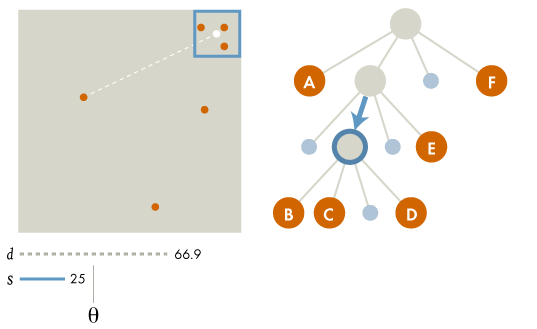
\includegraphics[width=\textwidth]{quadtree_internal}

\framebreak

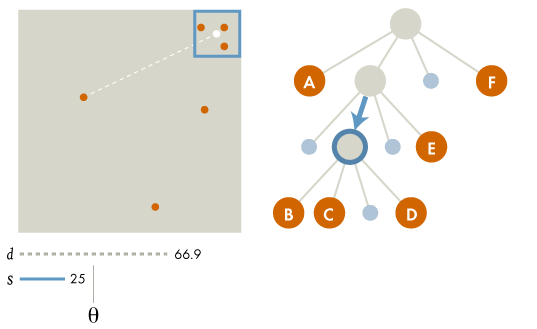
\includegraphics[width=\textwidth]{quadtree_internal}

\end{frame}

\section{Correctness}

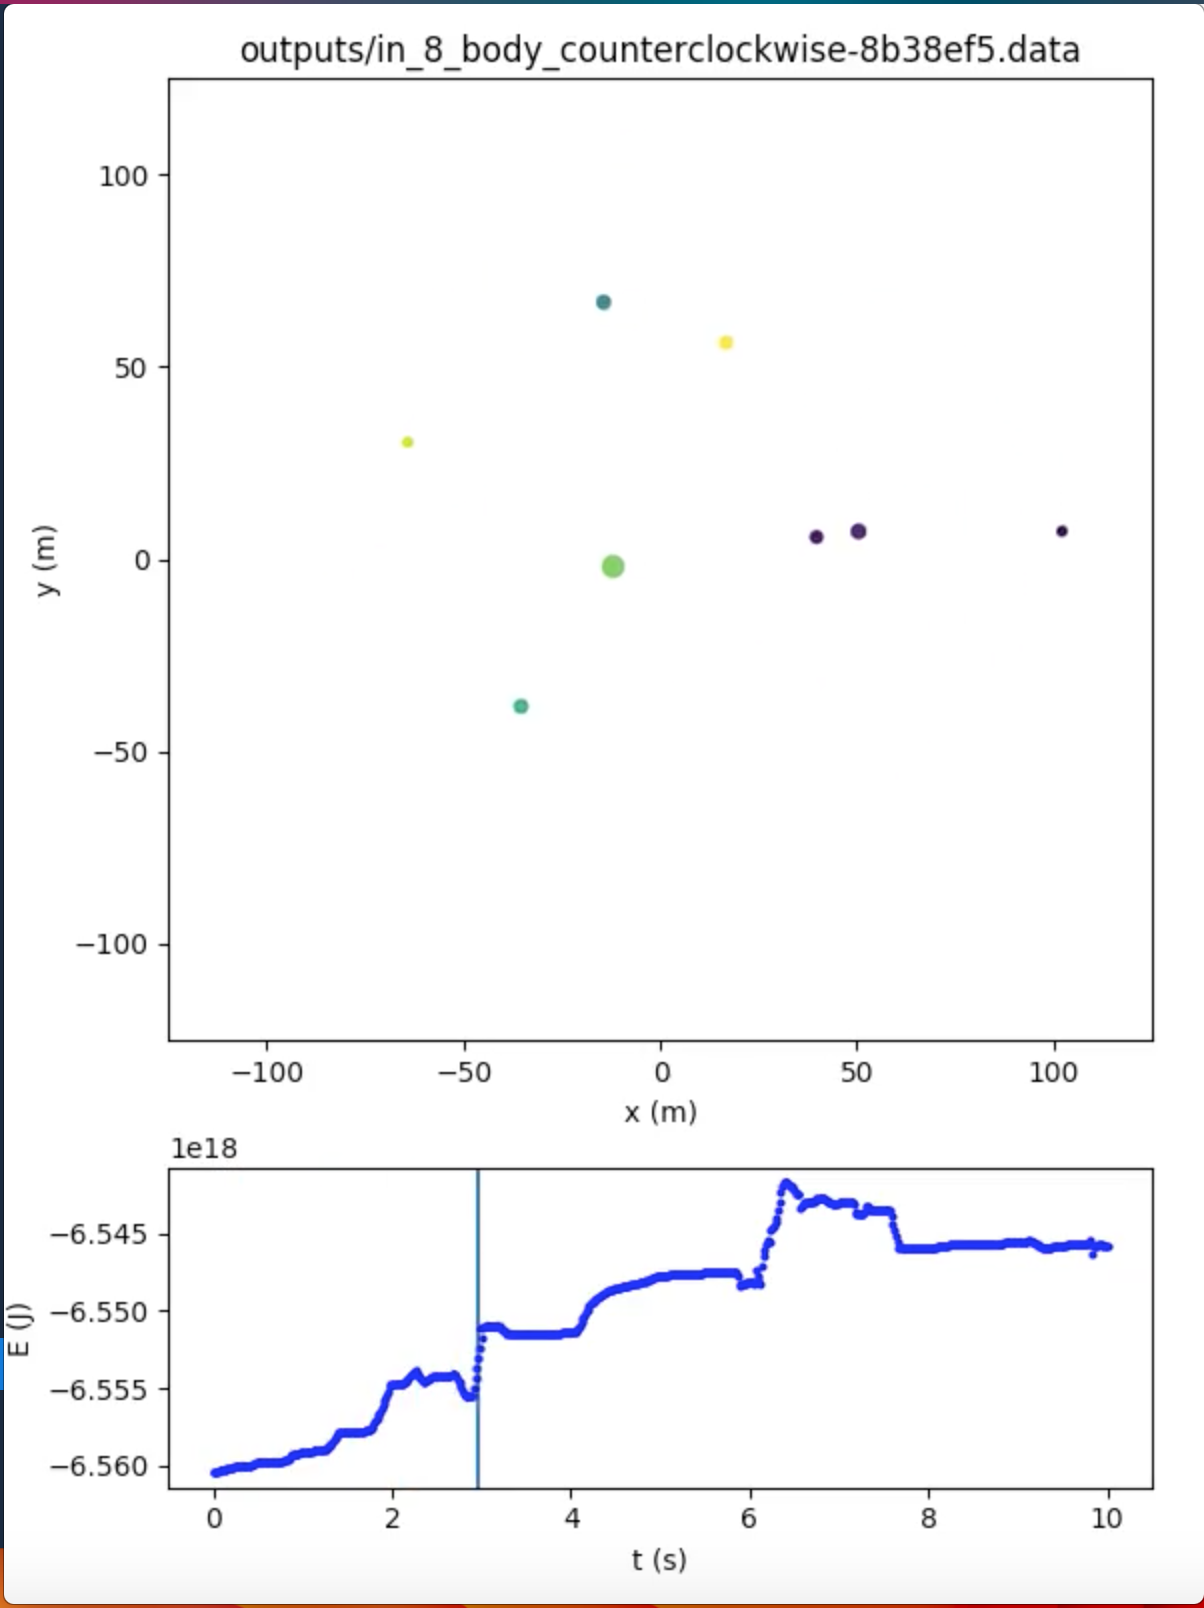
\includegraphics[width=\textwidth]{barnes_hut}

\framebreak

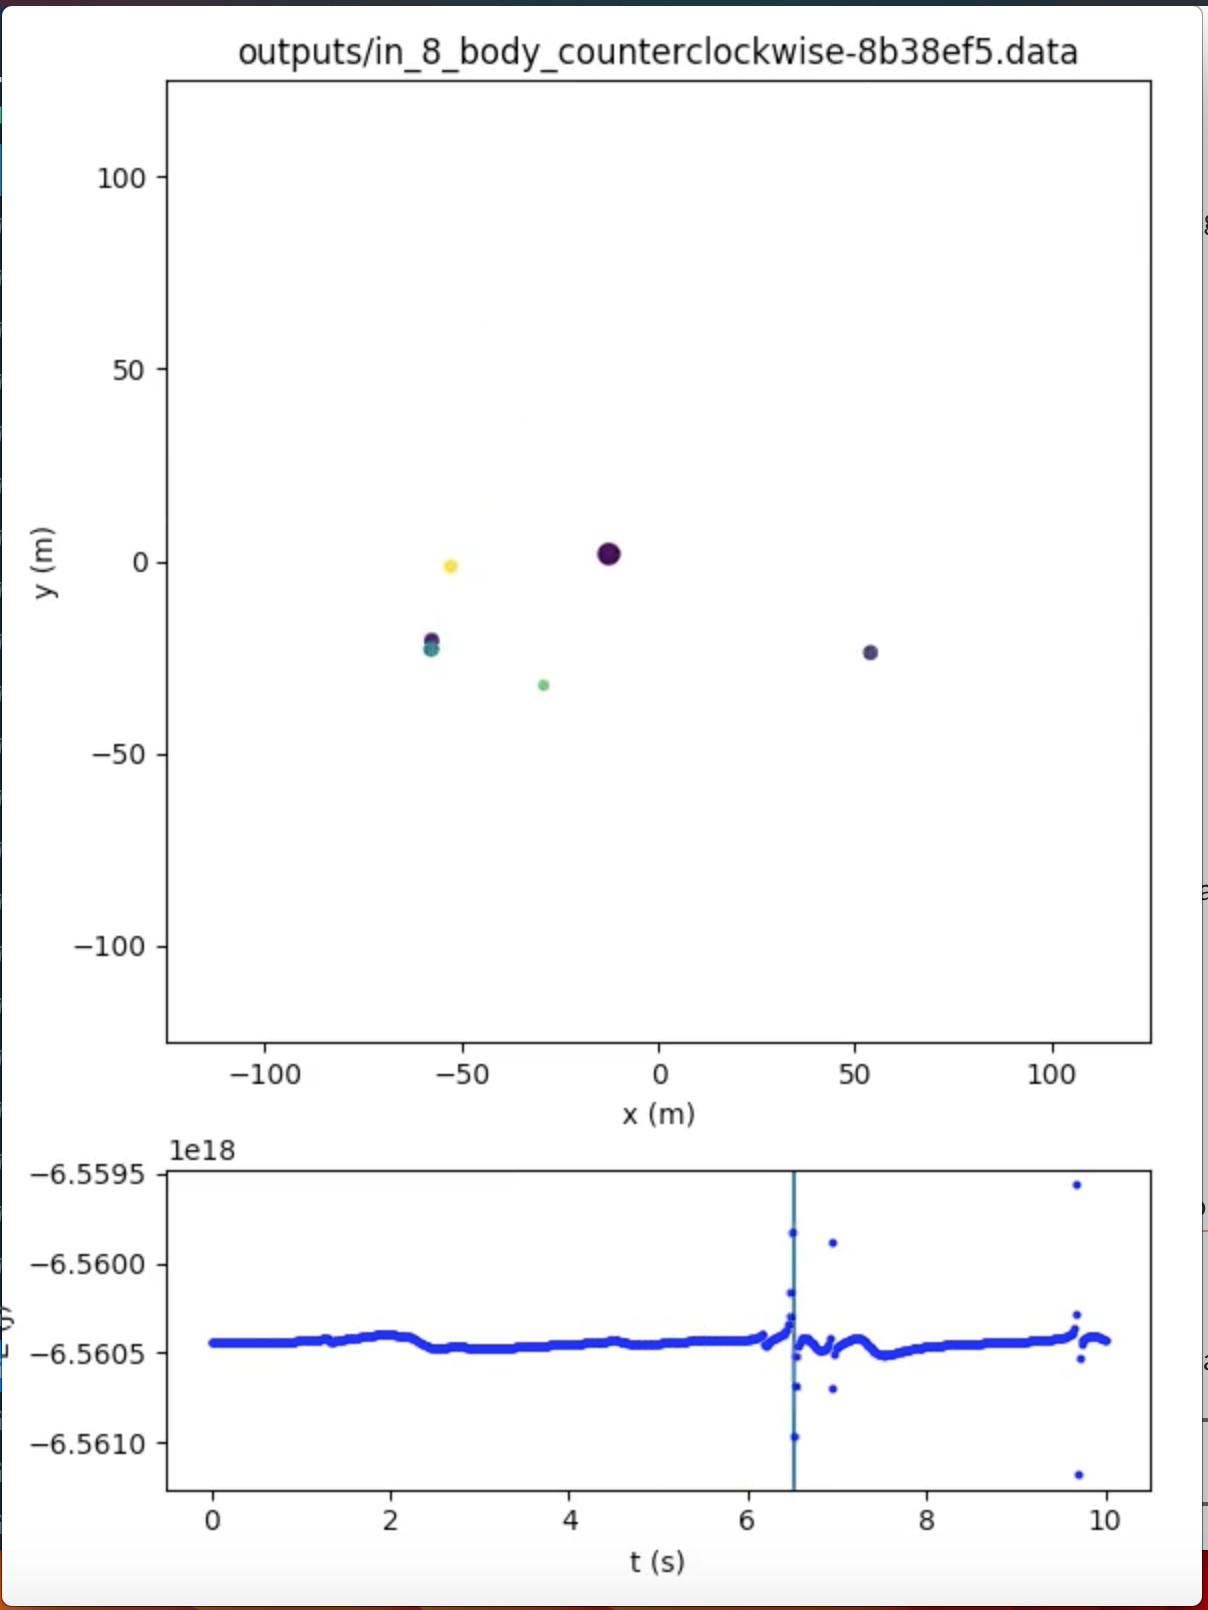
\includegraphics[width=\textwidth]{energy_anomaly}

\subsection{Tables and Figures}

\begin{frame}{Tables and Figures}

\begin{itemize}
\item Use \texttt{tabular} for basic tables --- see Table~\ref{tab:widgets}, for example.
\item You can upload a figure (JPEG, PNG or PDF) using the files menu. 
\item To include it in your document, use the \texttt{includegraphics} command (see the comment below in the source code).
\end{itemize}

% \begin{block}{Examples}
% Some examples of commonly used commands and features are included, to help you get started.
% \end{block}

% Commands to include a figure:
%\begin{figure}
%\includegraphics[width=\textwidth]{your-figure's-file-name}
%\caption{\label{fig:your-figure}Caption goes here.}
%\end{figure}

\begin{table}
\centering
\begin{tabular}{l|r}
Item & Quantity \\\hline
Widgets & 42 \\
Gadgets & 13
\end{tabular}
\caption{\label{tab:widgets}An example table.}
\end{table}

\end{frame}

\subsection{Mathematics}

\begin{frame}{Readable Mathematics}

Let $X_1, X_2, \ldots, X_n$ be a sequence of independent and identically distributed random variables with $\text{E}[X_i] = \mu$ and $\text{Var}[X_i] = \sigma^2 < \infty$, and let
$$S_n = \frac{X_1 + X_2 + \cdots + X_n}{n}
      = \frac{1}{n}\sum_{i}^{n} X_i$$
denote their mean. Then as $n$ approaches infinity, the random variables $\sqrt{n}(S_n - \mu)$ converge in distribution to a normal $\mathcal{N}(0, \sigma^2)$.

\end{frame}

\end{document}
